\documentclass[a4paper,11pt]{article}
\usepackage{amsmath,amsthm,amsfonts,amssymb,amscd,amstext,vmargin,graphics,graphicx,tabularx,multicol} \usepackage[french]{babel}
\usepackage[utf8]{inputenc}  
\usepackage[T1]{fontenc} 
\usepackage[T1]{fontenc}
\usepackage{amsmath,amssymb}
\usepackage{pstricks-add,tikz,tkz-tab,variations}
\usepackage[autolanguage,np]{numprint} 

\setmarginsrb{1.5cm}{0.5cm}{1cm}{0.5cm}{0cm}{0cm}{0cm}{0cm} %Gauche, haut, droite, haut
\newcounter{numexo}
\newcommand{\exo}[1]{\stepcounter{numexo}\noindent{\bf Exercice~\thenumexo} : \marginpar{\hfill /#1}}
\reversemarginpar


\newcounter{enumtabi}
\newcounter{enumtaba}
\newcommand{\q}{\stepcounter{enumtabi} \theenumtabi.  }
\newcommand{\qa}{\stepcounter{enumtaba} (\alph{enumtaba}) }
\newcommand{\initq}{\setcounter{enumtabi}{0}}
\newcommand{\initqa}{\setcounter{enumtaba}{0}}

\newcommand{\be}{\begin{enumerate}}
\newcommand{\ee}{\end{enumerate}}
\newcommand{\bi}{\begin{itemize}}
\newcommand{\ei}{\end{itemize}}
\newcommand{\bp}{\begin{pspicture*}}
\newcommand{\ep}{\end{pspicture*}}
\newcommand{\bt}{\begin{tabular}}
\newcommand{\et}{\end{tabular}}
\renewcommand{\tabularxcolumn}[1]{>{\centering}m{#1}} %(colonne m{} centrée, au lieu de p par défault) 
\newcommand{\tnl}{\tabularnewline}

\newcommand{\trait}{\noindent \rule{\linewidth}{0.2mm}}
\newcommand{\hs}[1]{\hspace{#1}}
\newcommand{\vs}[1]{\vspace{#1}}

\newcommand{\N}{\mathbb{N}}
\newcommand{\Z}{\mathbb{Z}}
\newcommand{\R}{\mathbb{R}}
\newcommand{\C}{\mathbb{C}}
\newcommand{\Dcal}{\mathcal{D}}
\newcommand{\Ccal}{\mathcal{C}}
\newcommand{\mc}{\mathcal}

\newcommand{\vect}[1]{\overrightarrow{#1}}
\newcommand{\ds}{\displaystyle}
\newcommand{\eq}{\quad \Leftrightarrow \quad}
\newcommand{\vecti}{\vec{\imath}}
\newcommand{\vectj}{\vec{\jmath}}
\newcommand{\Oij}{(O;\vec{\imath}, \vec{\jmath})}
\newcommand{\OIJ}{(O;I,J)}

\newcommand{\bmul}[1]{\begin{multicols}{#1}}
\newcommand{\emul}{\end{multicols}}


\newcommand{\reponse}[1][1]{%
\multido{}{#1}{\makebox[\linewidth]{\rule[0pt]{0pt}{20pt}\dotfill}
}}

\newcommand{\titre}[5] 
% #1: titre #2: haut gauche #3: bas gauche #4: haut droite #5: bas droite
{
\noindent #2 \hfill #4 \\
#3 \hfill #5

\vspace{-1.6cm}

\begin{center}\rule{6cm}{0.5mm}\end{center}
\vspace{0.2cm}
\begin{center}{\large{\textbf{#1}}}\end{center}
\begin{center}\rule{6cm}{0.5mm}\end{center}
}



\begin{document}
\pagestyle{empty}
\titre{Interrogation : Nombres relatifs (1)}{Nom :}{Prénom :}{Classe}{Date}

\begin{tabular}{|m{11cm}|c|c|c|}
\hline 
\textbf{Compétences} & \textbf{Acquis} & \textbf{En cours}  & \textbf{Non acquis} \\ 
\hline 
- Connaître la notion de nombre opposé. &  &  & \\
\hline
- Savoir ranger et comparer des nombres relatifs. &  &  &  \\ 
\hline 
- Connaître et utiliser le vocabulaire : origine,
coordonnées, abscisse, ordonnée.  &  &  &  \\ 
\hline 
- Dans le plan muni d'un repère orthogonal, savoir lire les coordonnées d'un point donné.  &  &  &  \\ 
\hline 
- Dans le plan muni d'un repère orthogonal, savoir placer un point de coordonnées données.  &  &  &  \\ 
\hline 


\end{tabular} 


\vspace*{1cm}



\exo{1,5} Cours : \\

\q Donner la définition d'un nombre relatif.\\
\reponse[3]\\




\q Quel est l'opposé de l'opposé de l'opposé de l'opposé de 4,8 ?\\
\reponse[1]\\





\exo{2,5}

\initq \q  Tracer une droite graduée de façon à pouvoir placer les points suivants :

E(-1,25)  \hspace*{0.5cm} R(0,75) 	 \hspace*{0.5cm}  S(-2,5) \hspace*{0.5cm} T(+1,75) \hspace*{0.5cm}  U(-0,5)\\
\vspace*{2.5cm}


\q  Tracer une autre droite graduée de façon à pouvoir placer les points suivants : 

A(+10) \hspace*{0.5cm} B(-15) \hspace*{0.5cm} L(-20) \hspace*{0.5cm} G(35)


\vspace*{2.5cm}
\exo{2,5} 

\initq \q Compléter les expressions suivantes avec les signes "<", ">" ou "=" :\\

-21  ......  - 23	 \hspace*{1.65cm}     23,2  ......  -14,2    \hspace*{1.65cm} 44,5  ......  44,05	\\   

-3,1  ......  -2,923 \hspace*{1cm} -1,99 ...... -1,999 \hspace*{1cm} -10,010 ...... -10,01\\

\q Ranger les nombres suivants dans l'ordre croissant : -18 ;  -2,45  ;  2,63 ;  -20  ;  -3  ; -1 ;  2,78 :  -2,5\\
\reponse[2]\\

\newpage


\exo{4}\\

\includegraphics[scale=1]{coordonnées.eps} \\

\initq \q Donner les coordonnées des points B, D et C.\\
\reponse[3]\\

\q Placer le point W tels que son abscisse est l'opposé de celle de D et son ordonnée est l'opposé de celle de E. \\

\q A l'aide du repère ci-dessus, placer les points suivants : G(4 ; 4) ; H(-5 ; 1) ; R(-3,5 ; 0) ; E( 0 ; 2,25 ) \\



\end{document}
